%    2. Write your answers in section "B" below. Precede answers for all 
%       parts of a question with the command "\question{n}{desc}" where n is
%       the question number and "desc" is a short, one-line description of 
%       the problem. There is no need to restate the problem.
%    3. If a question has multiple parts, precede the answer to part x with the
%       command "\part{x}".
%    4. If a problem asks you to design an algorithm, use the commands
%       \algorithm, \correctness, \runtime to precede your discussion of the 
%       description of the algorithm, its correctness, and its running time, respectively.
%    5. You can include graphics by using the command \includegraphics{FILENAME}
%
\documentclass[11pt]{article}
\usepackage{pgf}
\usepackage{tikz}
\usetikzlibrary{arrows,automata}
\usepackage{amsmath,amssymb,amsthm}
\usepackage{graphicx}
\usepackage[margin=1in]{geometry}
\usepackage{fancyhdr}
\usepackage{float}
\newcommand\ceil[1]{\lceil#1\rceil}
\setlength{\parindent}{0pt}
\setlength{\parskip}{5pt plus 1pt}
\setlength{\headheight}{13.6pt}
\newcommand\question[2]{\vspace{.25in}\hrule\textbf{#1}\vspace{.5em}\hrule\vspace{.10in}}
\renewcommand\part[1]{\vspace{.10in}\textbf{(#1)}}
\pagestyle{fancyplain}
\lhead{\textbf{\NAME\ (\UID)}}
\chead{\textbf{Homework Three}}
\rhead{CS 6966, \today}
\begin{document}\raggedright

\newcommand\NAME{Jake Pitkin}
\newcommand\UID{u0891770}
\newcommand\HWNUM{3}

\question{Problem 10}

Consider the simple experts setting: we have $n$ experts $E_1, ... \ ,E_n$, and each one makes a $0/1$ prediction each morning. Using these predictions, we need to make a prediction each morning, and at the end of the day we get a loss of $0$ if we predicted right, and $1$ if we made a mistake. This goes on for $T$ days.

Consider an algorithm that at every step, goes with the prediction of the `best' (i.e., the one with the least mistakes so far) expert so far. Suppose that ties are broken by picking the expert with a smaller index. Give an example in which this strategy can be really bad -- specifically, the number of mistakes made by the algorithm is roughly a factor $n$ worse than that of the best expert in hindsight.

\fbox{ \parbox{1\linewidth}{

We will show that given $n$ experts and this algorithm, we can construct an adversarial scenario where the algorithm makes a factor of $n$ more mistakes than the best expert. Consider the scenario where the true label is $0$ for all $T$ days. Each experts prediction is based on the following function of the current day $t$

$$
prediction_i(t) = \left\{
        \begin{array}{ll}
            1 & \quad t \ mod \ n = i - 1\\
            0 & \quad otherwise
        \end{array}
    \right.
$$

In this scenario the algorithm will make $T$ mistakes (always predicts wrong) and the best expert will be wrong $T / n$ number of times. \newline 

To give a concrete example, consider the scenario where we have $3$ experts and we run the algorithm for 9 days.

\begin{table}[H]
\centering
{\renewcommand{\arraystretch}{1.2}%
\begin{tabular}{| c | c | c | c | c | c | c | c | c | c |}
\hline
expert / $t$ & 0 & 1 & 2 & 3 & 4 & 5 & 6 & 7 & 8 \\ \hline
$E_1$ & 1 & 0 & 0 & 1 & 0 & 0 & 1 & 0 & 0 \\ \hline
$E_2$ & 0 & 1 & 0 & 0 & 1 & 0 & 0 & 1 & 0 \\ \hline
$E_3$ & 0 & 0 & 1 & 0 & 0 & 1 & 0 & 0 & 1 \\ \hline
true prediction & 0 & 0 & 0 & 0 & 0 & 0 & 0 & 0 & 0 \\ \hline
selected expert & $E_1$ & $E_2$ & $E_3$ & $E_1$ & $E_2$ & $E_3$ & $E_1$ & $E_2$ & $E_3$ \\ \hline
\end{tabular}}
\end{table}

We can see that in this example the algorithm always makes a mistake. Each expert is tied for being the best expert as they are each wrong $T/n$ or $3$ times. We have shown that this algorithm can make a factor of $n$ more mistakes than the best expert.

} }

\question{Problem 11}

We saw in class a proof that the VC dimension of the class of $n$-node, $m$-edge \textit{threshold} neural networks is $O((m+n)\log⁡ n)$. Let us give a ``counting'' proof, assuming the weights are binary $(0/1)$. (This is often the power given by VC dimension based proofs -- they can `handle' continuous parameters that cause problems for counting arguments).

\part{a} Specifically, how many ``network layouts'' can there be with $n$ nodes and $m$ edges? Show that $n(n-1)/2 \choose m$ is an upper bound.

\fbox{ \parbox{1\linewidth}{

From the text, we know a feedforward neural network is defined as a directed acyclic graph. It's known that the maximum number of edges a DAG can contain is $n(n - 1)/2$. To see this, the first node can point to all other nodes but itself, the next can point to all nodes other than itself and the first node and so on. 

$$(n - 1) + (n - 2) + ... + 2 + 1 = \sum_{i = 1}^{n - 1} i = \frac{n(n - 1)}{2}$$

Given the maximum number of edges a network can contain is $n(n - 1)/2$, we can observe that there exists at most $n(n-1)/2 \choose m$ network layouts with $n$ nodes and $m$ edges. Each distinct network layout is defined by \textit{choosing} $m$ edges from a maximum possible $n(n-1)/2$ edges. Thus, the binomial coefficient captures all possible network layouts and is an upper bound.

} }

\part{b} Given a network layout, argue that the number of `possible networks' is at most $2^m(n+1)^n$. [HINT: what can you say about the potential values for the thresholds?]

\fbox{ \parbox{1\linewidth}{

Given a network layout, the number of 'possible networks' is defined by the number of possible threshold and edge weight combinations. Consider a feedforward neural network with $n$ nodes and $m = n(n - 1)/2$ edges, which is the maximum number of edges a DAG can contain (as described in part a). \\

From the problem, we are assuming the weights are binary $(0/1)$. It follows that given $m$ edges, that can each take a value from $\{0, 1\}$, there are $2^m$ possible ways to select these weights. \\

The network is constructed such that node $n_i$ has an in-degree of $(n - i)$ (from the proof of constructing a DAG with the maximal number of edges). As such, node $n_i$ has a potential threshold value of $(n - i)$ as the edge weights can take a value from $\{0, 1 \}$. This gives

$$(n - 1) * (n - 2) + ... + 2 + 1 = \prod_{i = 1}^{n - 1} i = (n - 1)!$$

potential values for the thresholds. It is clear that $(n - 1)! < (n + 1)^n$. Thus, the number of 'possible networks' given by the feedforward neural network with the maximal number of edges (which maximizes the range of potential values for the thresholds) is upper bounded by $2^m(n+1)^n$.

$$2^m(n - 1)! \leq 2^m(n+1)^n$$

} }

\part{c} Use these to show that the VC dimension of the class of binary-weight, threshold neural networks is $O((m+n)\log ⁡n)$.

\fbox{ \parbox{1\linewidth}{

} }

\question{Problem 12 - Importance of Random Initialization}

Consider a neural network consisting of (resp.) the input layer $x$, hidden layer $y$, hidden layer $z$, followed by the output node $f$. Suppose that all the nodes in all the layers compute a `standard' sigmoid. Also suppose that every node in a layer is connected to every node in the next layer (i.e., each layer is fully connected).

Now suppose that all the weights are initialized to 0, and suppose we start performing SGD using backprop, with a fixed learning rate. Show that at every time step, all the edge weights in a layer are equal.

\fbox{ \parbox{1\linewidth}{
We suppose that all the weights $\mathbf{w}$ are initialized to $0$ before SGD is performed on the neural network. We will show that at every time step, all of the edge weights in a layer update by the same quantity keeping them equal. At each time step $t$ we sample $(\mathbf{x}, \mathbf{y}) \sim \mathcal{D}$, calculate the gradient $\mathbf{v_t}$ using the backpropagation algorithm and update the weights $\mathbf{w}$.\\ 

The input to the backpropagation algorithm is the sampled example $(\mathbf{x}, \mathbf{y})$, weight vector $\mathbf{w}$, the network $(V, E)$, and an activation function $\sigma$. In this example we have three hidden layers $x$, $y$, and $z$. During the \textit{forward step} of the backprop we set $\mathbf{o_0} = \mathbf{x}$ and calculate $a_{t,i}$ and $o_{t,i}$ in order where $t$ is the current hidden layer and $i$ is the node in that layer. The values for $a_{t,i}$ and $o_{t,i}$ are calculated as such:

$$a_{t,i} = \sum_{j = 1}^{k_{t-1}} \mathbf{w}_{t-1,i,j} * o_{t-1,j}$$
$$o_{t,i} = \sigma(a_{t,i})$$

The important observation here is all the weights $\mathbf{w}_{t-1,i,j}$ are zero causing all $a_{t,i}$ to be zero. As such, all $o_{t,i}$ (for a given $t$ or layer) with be equal. \\

During the \textit{backward step} these $o_{t,i}$ are used to calculate the partial derivatives that define the gradient

$$\delta_{t,i} = \sum_{j = 1}^{k_{t+1}} \mathbf{w}_{t,j,i} * \delta_{t+1,j} * \sigma^\prime(a_{t+1,j})$$

As such during the update step in SGD using the $\mathbf{v_i}$ gradients produced by backprop

$$\mathbf{w}^{(i + 1)} = \mathbf{w}^{(i)} - \eta(\mathbf{v_i} + \lambda\mathbf{w^{(i)})}$$

Will produce identical updates to the weights for each node in a layer. Thus all the edge weights in a layer stay equal at each time step $t$.

} }

\question{Problem 13}

Let us consider networks in which each node computes a rectified linear (ReLU) function (described in the next problem), and show how they can compute very `spiky' functions of the input variables. For this exercise, we restrict to one-variable.

\part{a} Consider a single (real valued) input $x$. Show how to compute a ``triangle wave'' using one hidden layer (constant number of nodes) connected to the input, followed by one output $f$. Formally, we should have $f(x) = 0$ for $x \leq 0$, $f(x) = 2x$ for $0 \leq x \leq 1/2$, $f(x) = 2(1 - x)$ for $1/2 \leq x \leq 1$, and $f(x) = 0$ for $x \geq 1$. [HINT: choose the thresholds and coefficients for the ReLU's appropriately.] [HINT2: play with a few ReLU networks, and try to plot the output as a function of the input.]

\fbox{ \parbox{1\linewidth}{
After some experimentation, I came up with a neural network with one hidden layer of size two that computes the given triangle wave function. \\

\begin{figure}[H]
\centering
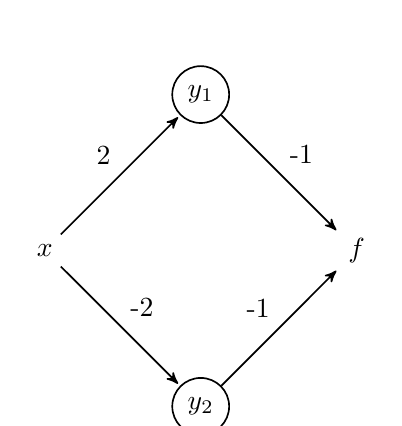
\begin{tikzpicture}[->,>=stealth',shorten >=1pt,auto,node distance=2.8cm,
                    semithick]

  \tikzstyle{every state}=[fill=white,draw=none,text=black]

  \node[]                     (A)                    {$x$};
  \node[draw, circle]         (B) [above right of=A] {$y_1$};
  \node[draw, circle]         (D) [below right of=A] {$y_2$};
  \node[]                     (C) [below right of=B] {$f$};

  \path (A) edge              node {2} (B)
  		(A) edge			  node {-2} (D)
        (B) edge              node {-1} (C)
        (D) edge              node {-1} (C);
\end{tikzpicture}
\end{figure}

Where $y_1$ and $y_2$ are threshold functions that take in the input weighted defined as such

$$
y_1(z) = \left\{
        \begin{array}{ll}
            z - 1 & \quad z > 1\\
            0 & \quad otherwise
        \end{array}
    \right.
$$
$$    
y_2(z) = \left\{
        \begin{array}{ll}
            z + 1 & \quad z > -1\\
            0 & \quad otherwise
        \end{array}
    \right.
$$

and the \textit{output} function $f$ is also a threshold function

$$    
f(z_1, z_2) = \left\{
        \begin{array}{ll}
            z_1 + z_2 + 1 & \quad z_1 + z_2 > -1\\
            0 & \quad otherwise
        \end{array}
    \right.
$$

This network is defining a composition of 3 ReLU functions, which as a function of $x$ can be expressed as such 

$$f(x) = max(0 , -max(0, 2x - 1) - max(0, -2x + 1) + 1)$$

\begin{figure}[H]
  \centerline{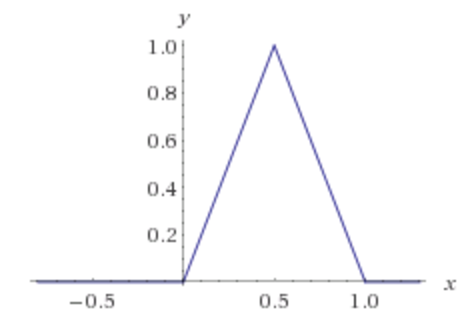
\includegraphics[width=0.5\linewidth]{13a.png}}
\end{figure}

} }

\part{b} What happens if you stack the network on top of itself? (Describe the function obtained). [Formally, this means the output of the network you constructed above is fed as the input to an identical network, and we are interested in the final output function.]

\fbox{ \parbox{1\linewidth}{
Taking the network from part a, we can stack the network on top of itself where $y_1$, $y_2$, and $f$ are defined as they are defined in part a

\begin{figure}[H]
\centering
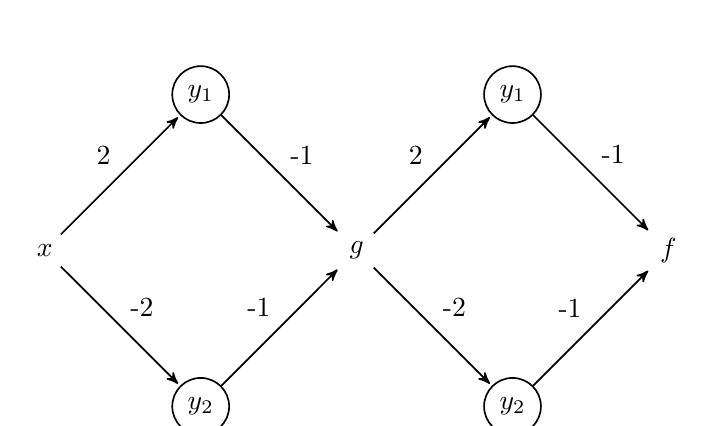
\begin{tikzpicture}[->,>=stealth',shorten >=1pt,auto,node distance=2.8cm,
                    semithick]

  \tikzstyle{every state}=[fill=white,draw=none,text=black]

  \node[]                     (A)                    {$x$};
  \node[draw, circle]         (B) [above right of=A] {$y_1$};
  \node[draw, circle]         (D) [below right of=A] {$y_2$};
  \node[]                     (C) [below right of=B] {$g$};
  \node[draw, circle]         (E) [above right of=C] {$y_1$};
  \node[draw, circle]         (F) [below right of=C] {$y_2$};
  \node[]         (G) [below right of=E] {$f$};

  \path (A) edge              node {2} (B)
  		(A) edge			  node {-2} (D)
        (B) edge              node {-1} (C)
        (D) edge              node {-1} (C)
        (C) edge			  node {2} (E)
        (C) edge			  node {-2} (F)
        (F) edge			  node {-1} (G)
        (E) edge			  node {-1} (G);
\end{tikzpicture}
\end{figure}

We can define $f(x)$ as a composition of $g(x)$ where $g(x)$ is the output of the initial network and becomes input for the identical second network

$$g(x) = max(0 , -max(0, 2x - 1) - max(0, -2x + 1) + 1)$$

$$f(x) = max(0 , -max(0, 2g(x) - 1) - max(0, -2g(x) + 1) + 1)$$

\begin{figure}[H]
  \centerline{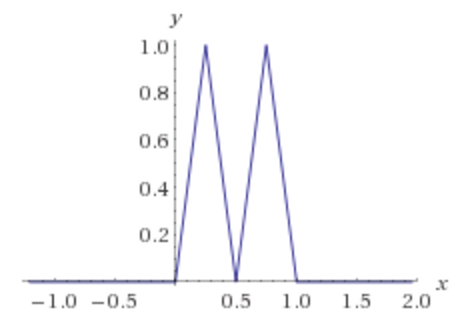
\includegraphics[width=0.5\linewidth]{13b.png}}
\end{figure}

} }

\part{c} Prove that there is a ReLU network with one input variable $x$, $2k+O(1)$ layers, all coefficients and thresholds being constants, that computes a function that has $2^k$ ``peaks'' in the interval $[0,1]$.

\fbox{ \parbox{1\linewidth}{
Using induction we will prove that as the number of layers in the ReLU network grows linearly the number of "peaks" in the interval $[0, 1]$ grows exponentially.\\ 

\textit{base case:} In \textit{part a} we constructed a ReLU network that had a single peak and O(1) layers ($k = 0$ and as such $2(0) + O(1)$ layers and $2^0 = 1$ peak).\\

\textit{inductive hypothesis:} For all ReLU networks with $2k + O(1)$ layers, the network contains $2^k$ peaks. \\

\textit{inductive step:} We will use the hypothesis that a ReLU network with $2k + O(1)$ layers contains $2^k$ peaks implies that a ReLU network with $2(k + 1) + O(1)$ layers contains $2^{k + 1}$ peaks. \\

Each peak $k$ in the network has a value of $1$ which can be observed by graphing the triangle wave function. Each time we add another copy of the network on top of itself (as seen in part b) the output of the previous "network" becomes the input for the new "network". We can observe an input of $1$ to the network produces an output of 0.

$$f(x) = max(0 , -max(0, 2x - 1) - max(0, -2x + 1) + 1)$$

As such each $k$ peak in the network becomes a valley when a new network is added to the overall network. Additionally, each $k$ peak outputs the value $0.5$ twice which will produce two new peaks in the overall network. The overall network gains $2$ layers each time we add an additional network stack and the number of peaks doubles. \\

Thus when a network contains $2(k + 1) + O(1)$ layers, it will contain $2^{k + 1}$ peaks. 
} }

\question{Problem 14}

In this exercise, we make a simple observation that width isn't as "necessary" as depth. Consider a network in which each node computes a rectified linear (ReLU) unit -- specifically the function at each node is of the form $max \{ 0,a_1y_1+a_2y_2+ ... +a_my_m + b \}$, for a node that has inputs $y1, ... \ ,ym$. Note that different nodes could have different coefficients and offsets ($b$ above is called the offset).

Consider a network with one (real valued) input $x$, connected to $n$ nodes in a hidden layer, which are in turn connected to the output node, denoted $f$. Show that one can construct a depth $n + O(1)$ network, with just 3 nodes in each layer, to compute the same $f$. [HINT: three nodes allow you to "carry over" the input; ReLU's are important for this.]

\fbox{ \parbox{1\linewidth}{

} }

\newpage

\question{Collaboration}

I collaborated with Sierra Allred, Maks Cegielski-Johnson, and Dietrich Geisler on problem 11, problem 12, and problem 13. \newline




\end{document}